\section{Assignments following discrete events}

In \sbmlLthreeVone, \class{EventAssignment}s are used to assign values to variables of a model, that are \class{Compartment}s, \class{Species}, \class{SpeciesReference}, or global \class{Parameter}s  when some conditions are fulfilled. In order to assign the value of a specific type of species, \class{EventAssignment}s in \multiVone also contain an element \class{SpeciesTypeInstanceChange}. The assignment sets the quantity of instances that fulfil a certain selection using the mathematical expression provided. 

\begin{figure}[h!]
\begin{center}
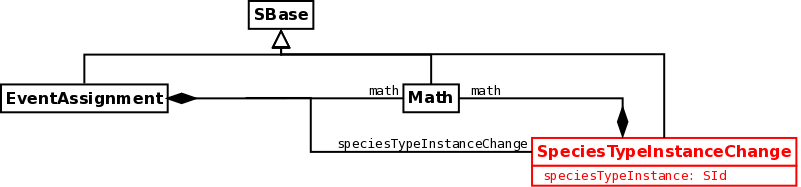
\includegraphics[scale=0.3]{./figs/pngs/EventAssignmentGeneral.png}
\caption{\class{EventAssignment} and all the associated classes of \multiVone.}
\end{center}
\end{figure}

\subsection{EventAssignment}

In order to assign values to entity subpools, defined by specific state and connectivity, following a discrete event, the element \class{eventAssignment} of \sbmlLthreeVone core is linked to a \class{SpeciesTypeInstanceChange}.

\begin{figure}[H]
\begin{center}
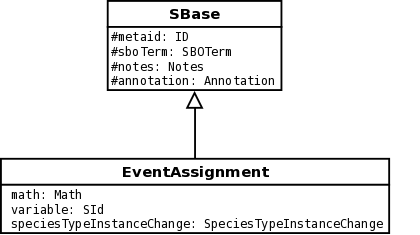
\includegraphics[scale=0.4]{figs/pngs/EventAssignmentClass.png} 
\caption{Definition of the extended version of \class{EventAssignment} and its relation with \class{SBase}.}
\label{fig:EventAssignmentClass}
\end{center}
\end{figure}

\subsection{SpeciesTypeInstanceChange}

For a definition of \class{SpeciesTypeInstanceChange}, see section \ref{SpeciesTypeInstanceChange}.